\chapter{Fundamentos da Matemática 1}

\section*{Recomendações Preliminares}
Algumas recomendações úteis:
\begin{itemize}
    \item Se inscreva no portal \url{https://pt.khanacademy.org/};
    \item Jogue jogos que envolvam raciocínio e tática como damas, xadrez, SUDOKU.
    \item Entre no portal \url{http://www.hypatiamat.com/} e jogue sempre que tiver tempo;
    \item Entre no portal \url{https://rachacuca.com.br/} para jogar jogos de raciocínio online;
    \item Baixe em seu computador o programa Geogebra.
    \begin{itemize}
        \item Navegue no portal \url{http://www.geogebra.im-uff.mat.br/index.html} e aprenda\linebreak como instalar o programa, ver como funciona através de vídeos tutoriais, além de acessar uma biblioteca com artigos sobre Geometria Dinâmica.
    \end{itemize}
    \item Se inscreva no portal \url{http://matematica.obmep.org.br/} e explore-o;
    \item Procure conhecer a coleção de Fundamentos da Matemática Elementar do Yezzi;
    \item Procure conhecer a coleção do Professor de Matemática da SBM;
\end{itemize}

\section{Revisão de Conjuntos}

\section*{Símbolos}

\begin{center}
\begin{tabular}{|c|c|}
\hline
$\in$ & pertence \\
\hline
$\not\in$ & não pertence\\
\hline
$\exists$ & existe \\
\hline
$\nexists$  & não existe \\
\hline
$\subset$  & está contido \\
\hline
$\not\subset$ & não está contido \\
\hline
$\forall$ & para todo \\
\hline
$\emptyset$  & conjunto vazio \\
\hline
$\supset$  & contém \\
\hline
$|$ & não está contido \\
\hline
$\longleftrightarrow $ & se e somente se \\
\hline
$\mathbb{N}$  & conjunto dos números naturais \\
\hline
$\mathbb{Z}$& conjunto dos números inteiros \\
\hline
$\mathbb{Q}$ & conjunto dos números racionais \\
\hline
$\mathbb{I}$ & conjunto dos números irracionais \\
\hline
$\mathbb{R}$ & conjunto dos números reais \\
\hline
\end{tabular}
\end{center}

\section{Relação de pertinência}

Cada aluno da classe tem uma mesma propriedade: estar na sala de aula. Assim, ao falarmos neste conjunto estabelecemos a possibilidade de averiguar se uma pessoa pertence ou não a ele. O conceito básico da teoria dos conjuntos é a relação de pertinência representada pelo símbolo $\in$. As letras minúsculas designam os elementos de um conjunto e as maiúsculas, os conjuntos. Assim, o conjunto das vogais $(V)$ é: $V = \{a, e, i, o, u\}$

\begin{itemize}
    \item A relação de pertinência é expressa por: $a \in V$, pois o elemento a pertence ao conjunto V.
    \item A relação de não-pertinência é expressa por: $b \not\in V$, pois o elemento b não pertence ao conjunto V.
\end{itemize}

\section{Formação de um conjunto}
Um conjunto pode ser definido de duas maneiras: enumerando seus elementos ou expressando uma ou mais propriedades que caracterízam todos os seus elementos.


\subsection{Enumerando elementos}
Aqui um conjunto seria expresso indicando cada um dos seus elementos. Por exemplo o conjunto $S$ a baixo.

 $S = \{1, 3, 5, 7, 9\}$
 
 Note que essa representação só é viável para o caso em que o conjunto é finito e, preferencialmente, com poucos elementos. Por exemplo temos os conjuntos que reunem soluções de equações. Uma equação de primeiro grau tem apenas uma solução. Uma equação quadrática tem até duas soluções.

\subsection{Expressando propriedades}

$S = \{\mbox{números ímpares de um algarismo}\}$ ou ainda
$S=\{x\in \mathbb{N};n=2x+1\mbox{ e } n\leq 9\}$

$B = \{x \in S / x \mbox{ tem a propriedade P}\}$; (lê-se: x pertence ao conjunto S tal que x possui a propriedade P).
O conjunto B é formado por todos os elementos de S que possuem a propriedade P.
Exemplo: $B = \{x \in \mathbb{N} / x < 8\} = \{0, 1, 2, 3, 4, 5, 6, 7\}$

Essa propriedade é conhecida no Raciocínio Lógico de Proposição Aberta. Uma proposição é uma afirmação a qual podemos sempre definir se seu valor lógico é Verdadeiro ou Falso. Para mais detalhes iremos dedicar uma seção no capítulo sobre Raciocínio Lógico com o tema Diagramas Lógicos.


\begin{defi}
Conjunto vazio: é um conjunto que não possui elementos. O conjunto vazio é representado por $\{ \ \}$ ou $\emptyset$.
\end{defi}

\begin{defi}
Subconjuntos: quando todos os elementos de um conjunto A qualquer pertencem a um outro conjunto B, diz-se, então, que A é um subconjunto de B, ou seja $$A\subset B$$.
\end{defi}

Observações:
\begin{itemize}
\item Todo o conjunto A é subconjunto dele próprio, ou seja $A\subset A$;
\item O conjunto vazio, por convenção, é subconjunto de qualquer conjunto, ou seja $\emptyset \in A$.
\item Se $A \subset B$ e $B\subset A$, então $A=B$.
\item Se $A \subset B$ e $B \subset C$, então $A\subset C$.
\end{itemize}

Logicamente podemos relacionar a inclusão de conjuntos com a implicação lógica. 

Seja a proposição $p(x):x$ é um número par e $q(x):x$ é um múltiplo de $4$. Temos duas proposições abertas. Serão verdadeiras ou falsas dependendo de quem dizemos ser $x$. Caso $x$ seja $6$, teremos que $p(6)$ será verdadeira enquanto $q(6)$ será falsa.

Perseba que todos os números multiplos de $4$ também são pares. Isso significa que $q\rightarrow p$ (lê-se ``$q$ implica $p$'').

Vamos colocar todos os números que tornam a proposição $q(x)$ verdadeira em um conjunto $Q$ e todos os que tornam a proposição $p(x)$ verdadeira em um conjunto $P$.

Teremos então:

$P=\{x\in \mathbb{N}; p(x)\}=\{0, 2, 4, 6, 8, \dots\}$

$Q=\{k\in \mathbb{N}; q(x)\}=\{0,4,8,12,16, \dots\}$

Teremos, $Q \subset P$, pois os multiplos de quatro é um subconjunto dos números pares.

Geralmente podemos aplicar conjuntos nas implicações lógicas e deduzir suas relações bem mais rápido que utilizando cálculo proposicional.

\section{Igualdade de conjuntos}

\subsection{Propriedades básicas}
Para todos os conjuntos $A$, $B$ e $C$, para todos os objetos $x\in U$, temos que:
\begin{enumerate}
    \item $A=A$;
    \item Se $A=B$, então $B=A$;
    \item Se $A=B$ e $B=C$, então $A=C$;
    \item Se $A=B$ e $x\in A$, então $x\in B$
    \item Se $A=B$ e $A\subset C$, então $B \subset C$.
\end{enumerate}

Dois conjuntos são igual se, e somente se, possuem exatamente os mesmos elementos não importando a ordem ou a repetição.

Dentro do raciocínio lógico teremos a dupla implicação. Ela é conhecida como ``se, e somente se...''. 

Seja p: x é um número multiplo de 2 e q: x é um número par.

Seja $P$ o conjunto dos números multiplos de 2 e $Q$ o conjunto dos números pares. 

Teremos que os conjuntos $P$ e $Q$ são iguais ($P=Q$), pois um número ser par implica que ele é multiplo de dois ($p \rightarrow q$) e um número ser multiplo de dois implica que ele é par ($q \rightarrow p$). Ou sejam um número é par se, e somente se, ele for multiplo de dois ($p\leftrightarrow q$).

\section{Conjunto complementar}

Complementar de $A$ com respeito a $R$ e é representada por $C^R_A = R - A$.

No caso dos alunos de uma classe, o conjunto complementar do conjunto dos alunos presentes à aula será formado pelos alunos ausentes à aula.


{\huge Observação}
\fbox{
\begin{minipage}{13cm}
Caso esteja claro em relação a quem é o complementar, então representamos o complementar de $A$ por $\bar{A}$
\end{minipage}
}

\section{Operações com conjuntos}

\begin{defi}   
União de Conjuntos: dados os conjuntos A e B, define-se como união dos conjuntos A e B ao conjunto representado por $A \cup B$, formado por todos os elementos pertencentes a A ou B, ou seja:
\end{defi}

\def\firstcircle{(0,0) circle (1.5cm)}
\def\secondcircle{(0:2cm) circle (1.5cm)}

\colorlet{circle edge}{blue!50}
\colorlet{circle area}{blue!20}

\tikzset{filled/.style={fill=circle area, draw=circle edge, thick},
    outline/.style={draw=circle edge, thick}}

\setlength{\parskip}{5mm}


\begin{figure}[h]

\centering
% Set A or B

\begin{tikzpicture}
    \draw[filled] \firstcircle node {$A$}
                  \secondcircle node {$B$};
    \node[anchor=south] at (current bounding box.north) {$A \cup B$};
\end{tikzpicture}

\caption{$A \cup B = \{x|x \in A\mbox{ ou }x\in B\}$}
\label{fig:uniao}
\end{figure}

%\def\firstcircle{(0,0) circle (0.5)}
%\def\secondcircle{(.7,0) circle (0.5)}

%\begin{tikzpicture}[xscale=2,yscale=2]

%\begin{scope}
%        \fill[blue] \firstcircle;
%        \fill[blue] \secondcircle;
        %\fill[blue] \thirdcircle;
%        \draw \firstcircle node[below] {$A$};
%        \draw \secondcircle node [above] {$B$};
        %\draw \thirdcircle node [below] {$C$};
%    \end{scope}


\begin{exe}
Ano: 2015 Banca: IBFC Órgão: MGS Prova: Nível Fundamental Incompleto

A união entre os conjuntos $A =\{ 0,1,2,3,4,5\}$ e $B = \{1,2,3,5,6,7,8\}$ é: 

\begin{multicols}{4}
\begin{enumerate}
    \item[a)] $\{0,1,2,3,5,6,7,8\} $
    \item[b)] $\{0,1,2,3,4,5,6,7,8\} $
    \item[c)] $\{1,2,3,4,5,6,7,8\} $
    \item[d)] $\{0,1,2,3,4,5,6,8\} $
\end{enumerate}
\end{multicols}
\end{exe}


\begin{defi}
Intersecção de Conjuntos: dados os conjuntos A e B, define-se como intersecção dos conjuntos A e B ao conjunto representado por $A\cap B$, formado por todos os elementos pertencentes a A e B, simultaneamente, ou seja:  

\end{defi}



\begin{figure}[h]
\centering

% Set A and B
\begin{tikzpicture}
    \begin{scope}
        \clip \firstcircle;
        \fill[filled] \secondcircle;
    \end{scope}
    \draw[outline] \firstcircle node {$A$};
    \draw[outline] \secondcircle node {$B$};
    \node[anchor=south] at (current bounding box.north) {$A \cap B$};
\end{tikzpicture}

\caption{$A\cap B=\{x|x\in A\mbox{ e }x\in B\}$}
\label{fig:my_label}
\end{figure}

\subsection{Número de Elementos da União}

$$n(A \cup B)=n(A)+n(B)-n(A\cap B)$$

\begin{defi}
Diferença de Conjuntos: dados os conjuntos A e B, define-se como diferença entre A e B (nesta ordem) ao conjunto representado por $A-B$, formado por todos os elementos pertencentes a A, mas que não pertencem a B, ou seja: 
\end{defi}

\begin{figure}[h]
\centering

%Set A or B but not (A and B) also known a A xor B
\begin{tikzpicture}
    \begin{scope}
        \clip \firstcircle;
        \draw[filled, even odd rule] \firstcircle node {$A$}
                                     \secondcircle;
    \end{scope}
    \draw[outline] \firstcircle
                   \secondcircle node {$B$};
    \node[anchor=south] at (current bounding box.north) {$A - B$};
\end{tikzpicture}

\caption{$A-B=\{x|x\in a\mbox{ e }x\not\in B\}$}
\label{fig:my_label}
\end{figure}

\begin{center}
 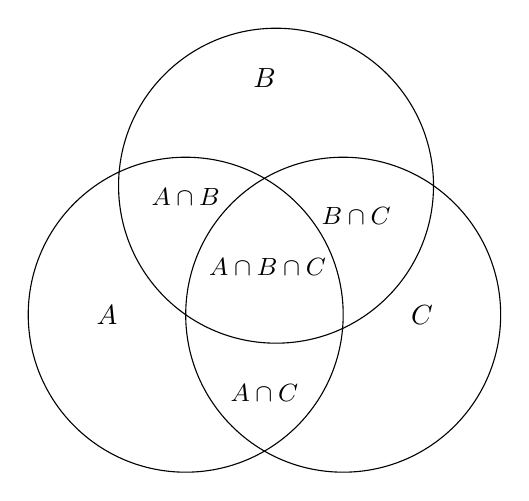
\begin{tikzpicture}

 \pagestyle{empty}

\def\firstcircle{(0,0) circle (2cm)}
\def\secondcircle{(55:2cm) circle (2cm)}
\def\thirdcircle{(0:2cm) circle (2cm)}

    \begin{scope}
      \clip \firstcircle;
      \clip \secondcircle;
      \fill[white] \thirdcircle;
    \end{scope}

    \draw \firstcircle;
    \node at (-1,0) {$A$};
    
    \draw \secondcircle;
    \node at (1,3) {$B$};
    
    \draw \thirdcircle;
    \node at (3,0) {$C$};
    
    \begin{scope}[font=\small]
     \draw(1,-1) node {$A\cap C$};
     \draw(90:1.5cm) node {$A\cap B$};
     \draw(30:2.5cm) node {$B\cap C$};
     \draw(30:1.2cm) node {$A\cap B\cap C$};
    \end{scope}
  \end{tikzpicture}
\end{center}


\begin{defi}
Produto Cartesiano: dados os conjuntos A e B, chama-se peoduto cartesiano A com B, ao conjunto $A\times B$, formado por todos os pares ordenados $(x,y)$, onde x é elemento de A e y é elemento de B, ou seja $$A\times B=\{(x,y)|x\in A\mbox{ e }y\in B\}$$ 
\end{defi}

%\subsection{Número de elementos - Probabilidade}
%\subsection{Número de elementos - Relacionado a porcentagem}

\subsection{Simplificação no cálculo proposicional}
A linguagem de conjuntos pode ser utilizado para simplificar e efetuar calculos lógicos. Como um conjunto pode ser definido como a coletividade de elementos de um certo universo predeterminado que satisfazem a uma proposição aberta bem definida. Por exemplo, no universo dos números naturais poderemos estabelecer o conjunto dos pares apenas tomando os elementos de $\mathbb{N}$ que tornam a proposição aberta ``\textit{P(x):x pode ser dividido por $2$}'' verdadeira.

Vejam que as operações entre conjuntos podem ser compreendidas como operações lógicas. Sendo assim uma equação proposicional pode ser modelada através de relações e operações entre conjuntos.



Agora vamos tomar um conjunto formado pelos números naturais menores ou iguais a um certo \textit{n}\footnote{$\{n,i\in \mathbb{N}; i\leq n\}$} e o representamos por $I_n=\{1,2, \dots, n\}$. Ou seja:

\begin{align*}
    I_1&=\{1\}\\
    I_2&=\{1,2\}\\
    I_3&=\{1,2,3\}\\
    \vdots &= \vdots \\
    I_n&=\{1,2,3, \dots , n\}
\end{align*}

\section*{Questões optativas}
\begin{enumerate}
\item Note que $I_1$ é subconjunto de $I_2$. E que $I_2$ é subconjunto de $I_3$. Logo temos que $I_1$ também é sunconjunto de $I_3$. Podemos generalizar e dizer que $I_n$ sempre será subconjunto de $I_m$ em que situração?

\item Note que a união de $I_1$ com $I_2$ é igual a $I_2$. E que a união de $I_2$ com $I_3$ é igual a $I_3$ (verifique). $I_1$ unido com $I_3$ será igual a quem? Quando eu posso dizer que a União de $I_n$ com $I_m$ é igual a $I_m$?

\item Quanto a intersecção de dois deles, relacione $I_1$ com $I_2$, depois $I_2$ com $I_3$ e depois $I_1$ com $I_3$. Quando que $I_n \cap I_m = I_m$?
\end{enumerate}

Note que o \textit{n} ao mesmo tempo que serve de indice para o conjunto \textit{I} ele diz quantos elementos tem em I (verifique).


Para o conjunto sem elementos temos temos que ele contem apenas um subconjunto, ele próprio. Para um sonjunto unitário ele possui dois sunconjuntos, um unitário e um vazio. Para um conjunto com dois elementos temos quatro subconjuntos: um vazio, dois unitário e um com dois elementos que é ele próprio. Seguindo essa orientação temos a seguinte tabela abaixo.\\

\begin{center}
  \begin{tabular}{|c|c|c|c|}
  \hline
       $A$  & $P(A)$ & Pascal &$|P(a)|$  \\
\hline
       $\{1\}$ & $\{ \emptyset , \{1\} \}$ & 1 \quad 1 & 2\\
\hline
$\{1,2\}$ & $\{ \emptyset , \{1\},\{2\}, \{1,2\} \}$ & 1 \quad 2 \quad 1 & 4\\
\hline
$\{1,2,3\}$& $\{ \emptyset , \{1\},\{2\},\{3\}, \{1,2\},\{1,3\},\{2,3\},\{1,2,3\} \}$ & 1 \quad 3 \quad 3 \quad 1  & 8\\
\hline

    \end{tabular}
\end{center}

A primeira coluna da matriz representa um conjunto $A$ qualquer com apenas um elemento na primeira linha, dois na segunda e assim por diante. Note que as regras para a quantidade de elementos e a forma de encontrar as partes desse conjunto não varia se forem mudados as espécies dos elementos de $A$, apenas se mudarem sua quantidade.

Na segunda coluna temos o conjunto das partes do conjunto $A$. Note que esse conjunto sempre contém o conjunto vazio e o próprio conjunto $A$. Sua composição será de todos os subconjuntos de $A$. Logo sua composição irá variar com subconjuntos vazio, com um elemento, dois elementos, etc até a quantidade total dos elementos de $A$ que é quando o próprio $A$ está contido nele. Mas a sua distribuição em relação a esses conjuntos é dada pela terceira coluna.

A terceira coluna que chamei de "Pascal" enumera em seu primeiro termo a quantidade de conjuntos vazios (sempre 1), en seu segund termo a quantidade de conjuntos unitários (1 na primeira linha, 2 na segunda, etc), no terceiro termo temos a quantidade de conjuntos com dois elementos. Ou seja, para o n-ésimo termo (quando o tiver) ele indicará a quantidade de subconjuntos de $A$ com $n-1$ elementos.

A quarta coluna indica a quantidade total dos elementos das partes do conjunto $A$. Note que há um padrão nessa numeração. Qual padrão é esse?



\begin{defi}
Número de subconjuntos de um conjunto: se um conjunto A possuir n elementos, então existirão $2^n$ subconjuntos de A.
 \end{defi}
 

 \begin{center}
$\begin{matrix} 1 \\ 1 \quad 1 \\ 1 \quad 2 \quad 1 \\ 1 \quad 3 \quad 3 \quad 1 \\ 1 \quad 4 \quad 6 \quad 4 \quad 1 \\ 1 \quad 5 \quad 10 \quad 10 \quad 5 \quad 1 \\ 1 \quad 6 \quad 15 \quad 20 \quad 15 \quad 6 \quad 1 \\ 1 \quad 7 \quad 21 \quad 35 \quad 35 \quad 21 \quad 7 \quad 1 \\ 1 \quad 8 \quad 28 \quad 56 \quad 70 \quad 56 \quad 28 \quad 8 \quad 1 \\ 1 \quad 9 \quad 36 \quad 84 \quad 126 \quad 126 \quad 84 \quad 36 \quad 9 \quad 1 \\ 1 \quad 10 \quad 45 \quad 120 \quad 210 \quad 252 \quad 210 \quad 120 \quad 45 \quad 10 \quad 1 \\ 1 \quad 11 \quad 55 \quad 165 \quad 330 \quad 462 \quad 462 \quad 330 \quad 165 \quad 55 \quad 11 \quad 1 \\ 1 \quad 12 \quad 66 \quad 220 \quad 495 \quad 792 \quad 924 \quad 792 \quad 495 \quad 220 \quad 66 \quad 12 \quad 1 \end{matrix}$
\end{center}

\section{Revisão de Equações}
O objetivo é revisar equações com uma introdução as funções. 

Lembre-se que uma expressão aritmética pode ser tanto uma função como uma equação. Note ainda que a equação nada mais é que um caso espefícifo da função. Quando temos uma expressão igualada a zero temos o ponto em que a função toca o eixo $x$.

\subsection{Equação do Primeiro Grau}
Faça diversas equações para valores consecutivos para, assim, introduzir a função pela \linebreak Progressão Aritmética. Contextualize com a função horária das posições para o movimento retilíneo uniforme e uniformemente variado para mostrar que a posição inicial seria o primeiro termo, a razão seria a velocidade e a posição final seria o termo geral.

\subsection{Equação do Seundo Grau}

Uma equação é toda igualdade em que de um lado temos uma expressão algébrica e do outro um resultado. No caso das equações quadráticas (outro nome dado para as equações do $2^o$ grau), teremos de uma expressão polinomial de grau dois igualado a zero.

\begin{equation}\label{1.1}
    ax^2+bx+c=0
\end{equation}

Para a resolução de equações desse gênero é conhecida fórmula de báscara que visa obter o valor das raízes em função dos coeficientes $a$, $b$ e $c$. A fórmula em questão é a de Bhaskara\footnote{Matemático Indiano do Século XII} e é expressa por

\begin{equation}\label{1.2}
    x=\dfrac{-b \pm \sqrt{\Delta}}{2a}
\end{equation}

em que $\Delta$ é o discriminante, e vale
\begin{equation}\label{1.3}
    \Delta=b^2-4ac.
\end{equation}

A fórmula acima pode ser deduzida a partir do processo de completar quadrado sobre a equação \eqref{1.1}.

\begin{exe}
Encontre o resultado da equação quadrática $2x^2-3x-1=0$
\end{exe}
O primeiro passo é identificar os coeficientes. 
\begin{align*}
    a&=2\\
    b&=-3\\
    c&=1
\end{align*}

Assim que identificamos os coeficientes passamos para encontrar o valor do discriminante.

\begin{align*}
    \Delta&=(-3)^2-4\cdot 2 \cdot 1\\
    &=9-8=1
\end{align*}

Basta agora substituir os valores do discriminante e dos outros termos em \eqref{1.2}.

\begin{align*}
    x&=\dfrac{-(-3)\pm \sqrt{1}}{2\cdot 2}\\
    &=\dfrac{2\pm 1}{4}
\end{align*}    
 
 Como o valor do discriminante é maior que zero teremos duas soluções diferentes.
 \begin{align*}
    \begin{cases}
    x'=\frac{3}{4}\\
    x''=\frac{2}{4}=\frac{1}{2}
    \end{cases}
 \end{align*}
 
 Para os casos em que o discriminante é zero, então teremos uma única solução. Quando o discriminante é negativo nós não teremos soluções reais.
 
 Apesar de podermos utilizar esse método para resolver quaisquer equações quadráticas, podemos economisar tempo em casos especiais.
 
 \subsection{Caso em que $b=0$}
 Nesse tipo de caso a equação \label{1.1} torna-se
 
 \begin{equation}\label{1.4}
     ax^2+c=0.
 \end{equation}
 Para esse tipo de situação basta isolar o termo quadrático e, por fim, retirar a raiz quadrada.
 
 \begin{align*}
     ax^2&=-c\\
     x^2&=-\dfrac{c}{a}\\
     x&=\pm \sqrt{-\dfrac{c}{a}}
 \end{align*}
 
 Geometricamente podemos representar esse caso com a figura abaixo
 
 FIGURA REPRESENTATIVA DE DIFERENÇA DE QUADRADOS
 
 
 \subsection{Caso e que $c=0$}
 Nesse caso a equação \label{1.1} torna-se
 
 \begin{equation}\label{1.5}
     ax^2+bx=0.
 \end{equation}
 
 Aqui podemos isolar o valor de $x$. Ficamos com 
 
 \begin{align*}
     x(ax+b)=0     
 \end{align*}
 
 que tem como solução apenas $x=0$ e $x=\frac{-b}{a}$.

REPRESENTAÇÃO GEOMÉTRICA
Função horária das posições para o movimento uniformemente variádo.

Progressão aritmética de segunda ordem. Problemas com sequências numéricas.

\section{Introdução as Funções}